\section{Background of the Study}


Understanding human behavior has been one of the most prevalent topic in implementing different applications. One of these human behaviors include Eye Gaze Estimation, where eye tracking technology is used to be able to determine the direction of the gaze of the eyes. Studying this human behavior can have extended applications such as research on psychology, study on the behavior of people with disabilities, analyzing behaviors of drivers, security monitoring, and human-computer interfaces.

There are researches already being conducted in order to minimize the number of devices and models used to implement eye gaze estimation. However, current methods are still requiring to have additional devices to be used. Eye gaze estimation could be done using an RGB-D camera wherein informations such as the depth or distance and the texture could be obtained, where these information are integrated and obtained just by using a kinect.

RGB-D camera capture and shows colored images as well as its depth which helps in 3-D representations and modelling. These cameras augment the usual images with its depth information. The augmentation happens in per-pixel basis. The RGB-D camera to be used in this study will be the Microsoft Kinect. This camera is useful because it is included in the line of motion sensing devices made by a reputable technological company. It makes use of natural user interface to capture images.

One way of determining whether an automobile driver is feeling drowsy or distracted is by observing the eye behaviour. According to Verwey, W.B., and Zaidel, D. M., one of the significant eye metrics that determines whether a driver is feeling drowsy is the frequency of eye closure exceeding one second whereas shorter ones are considered as blinks. The researchers intend to do the same thing with regards to evaluating driver drowsiness by observing the eyes, if either one or both of the eyes are closed. Eye gaze estimation is used for evaluating whether the driver is distracted or not.

The paper presents the use of Kinect as the RGB-D camera to track eye gazing by using the algorithm from the thesis Eye-Model-Based Gaze Estimation by RGB-D Camera by Jianfeng, L. and Shigang, L. The Kinect sensor is able to acquire the pose and 3D position of the head whereas the problem to be solved is detecting the pupil center of by obtaining it from the 3D eye model. The basis research showed promising results with little error in the algorithm of pupil centering. In addition, the researchers will be implementing the application of driver drowsiness detection that will alert the driver whenever they are positive of drowsiness.

\section{Prior Studies}

The use of eye tracking in daily lives of people is becoming ubiquitous. There have been studies that make use of eye tracking for different applications such as personality tests, focus and attention analysis, and even used in the automotives industry. There have been studies about eye tracking and its general applications. The applications presented include scientific and academic research, market research, neuroscience and psychology, psychology research, medical research, usability research, packaging research, pc and gaming research, human factors and simulation, and ophthalmology (Punde et. al., 2017). 

There were also studies that made use of eye tracking in order to study and analyze data from vehicle drivers. The data gathered and analyzed can be used in order to improve road safety and security as well as prevention of road accidents. Programming softwares such as MATLAB was used in order to test driver’s awareness and detect drowsiness in real-time. The addition of an alarm system for drivers will ensure that they can be alerted and reminded. 

The data used in these researches came from a large database known as GazeCapture as well as manually captured with the use of different kinds of cameras such as RGB-D and even webcam. The use of webcam is essentially focused on simplicity because it is already integrated in some devices such as laptops. On the other hand, the use of RGB-D camera in some researches showed that the accuracy and quality of images have improved. The microcontrollers used in past researches include Arduino and Raspberry Pi. These microcontrollers were used because of their simplicity, low cost, and low power consumption. The use of microcontrollers was utilized in past researches because algorithms can be programmed easily using applicable softwares.


\section{Problem Statement}

The ideal scenario in using an eye tracking device for driver awareness is to use a laptop for processing the image because it is faster and the device would be able to alert the driver in time before an accident assuming the driver became aware of the alert and was able to prevent the accident from happening.

The use of laptops for implementation of the eye tracking device in automobiles might be impractical due to its size. The researchers propose the use of microcontrollers to solve this problem. Although the use of microcontrollers would limit the robustness of the device. Microcontrollers have lower memories than a laptop therefore there would be less codes that can be embedded and the execution of codes are slower. The researchers would look for the optimal setup both in hardware and the software so that it would still be usable and could be improved for further researches.

Also the size of the kinect might be a hindrance to the view of the driver and might violate the RA 10913, which is the Anti-Distracted Driving Act. The solution to this is to place the kinect in a place where it can be mounted in accordance to the Anti-Distracted Driving Act.


\section{Objectives}

The main objective of the proposed thesis is to implement eye tracking technology for detecting driver’s awareness. The general and specific objectives are as follows:

\subsection{General Objective(s)}
To use a RGB-D camera for capturing the image in need of image processing for detecting eyes and driver’s awareness.

To implement an algorithm for detection of driver’s awareness based on eye behaviour.

To use existing algorithms for face pose estimation, pupil center estimation, head pose estimation, and eye gaze estimation

To create a standalone microcontroller based eye tracking device for detecting driver awareness


\subsection{Specific Objectives}

\begin{enumerate}
	
	\item To interface the microcontroller and RGB-D camera using MATLAB and SIMULINK
	
	\item To make use of MATLAB’s libraries for successfully creating a driver awareness algorithm 
	
	\item To make use of microsoft kinect as the RGB-D camera
	
	\item smoke weed everyday
	
	\item i love dicks
	
\end{enumerate}



\section{Significance of the Study}

Knowing how the human eye behaves in different situations and time shows a number of things about a given situation. The detection of where the eyes look at is helpful in determining one’s focus and attention. Moreover, the regions within the eyes’ sight that are ignored will also be known. Additional capabilities of eye trackers include detecting drowsiness, consciousness, and other mental states. The integration of these eye trackers to available electronic devices such as computers and mobile phones helps in analysis of consumer’s behavior and may lead to further technological advancements. In addition, almost every work and actions require visual information that is why eye tracking is very significant. The list of applications grows as time passes. Eye tracking technology also helps in researches and designs of fields including automotives, medical, defense, and entertainment industries. 

By understanding the user’s eye behavior, new safety and security measurements may be designed. In addition, there will be improvements on existing work based on data gathered from the eye movements and gaze patterns. The beneficiaries of this study include the user, the society and industries that make use of visual data for improvements, and future researchers as well. The user and the industries that continue to improve their products and devices help each other in such a way that the safety, security, and satisfaction of the users will be achieved given that their visual data and gaze patterns will be carefully analyzed by different industries. This study also helps in improving and testing of existing algorithms for eye tracking. Thus, this study will be of great help to future researchers that will engage and tackle this topic because eye tracking is important and significant in this modern age. 




\section{Assumptions, Scope and Delimitations}

This section provides the assumptions, scope, and delimitations of the research which serves as the guideline of how the research was done

\subsection{Assumptions}
\begin{enumerate}
	
	\item It is assumed that there are more people feeling sleepy at night therefore causing drowsy driving
	
	\item If either one or both of the eyes detected are evaluated as closed, then the driver is drowsy and an alarm system will turn on.
	
	\item If the pupil of the eyes is not located at the center, then the driver is distracted and an alarm system will turn on.
		
\end{enumerate}

\subsection{Scope}
\begin{enumerate}
	
	\item Create an algorithm for detection of driver’s awareness based on eye behaviour.
	
	\item Device should be available even on low light conditions because of the first assumption.
	
	\item To test for driver’s drowsiness, the device should be able to detect whether one or both of the eyes are closed.
	
	\item Can measure the blink rate of the eyes as an additional parameter in determining whether the driver is drowsy or not.
	
	\item Can detect whether driver is distracted by using pupil center estimation
		
\end{enumerate}

\subsection{Delimitations}
\begin{enumerate}
	
	\item Existing algorithms on eye detecting is used.
	
	\item Built in face detection algorithm provided by the Kinect Microsoft is used.
	
	\item In the pupil center estimation, the Kinect Microsoft had a difficulty with detecting the pupil when the driver is looking downward.
	
	\item The device had a difficulty in detecting eyes for people with small eye openings.
		
\end{enumerate}

\section{Description and Methodology}

Visual data will be gathered using RGB-D camera. The data gathered will be used by the eye tracker that follows a specific algorithm for each step of eye tracking. This eye tracker will be used to study and analyze the driver’s eye movements. Moreover, there will be an alarm system when the eye tracker detects fatigue, drowsiness, or other states which are not suited for driving a vehicle. The eye tracker will be placed in a position that does not block the driver’s vision of the road and other vehicles. In addition, the eye tracker’s placement is at a position permitted by the law.

The head pose is estimated using the kinect sensor and a head coordinate system is generated. Using the pupil center estimation algorithm, the 2D position of the pupil center will be taken and then translated later to 3D provided by the RGB-D camera, kinect sensor. Calibration will then take place by detecting the eyeball center. After the pupil center and eyeball center locations have been known, the gaze direction can be estimated.

Using MATLAB and SIMULINK, an algorithm will be made for the evaluation whether the driver is drowsy or distracted and alarm system will sound to alert the driver. It will also be used to interface the materials such as the Microsoft Kinect, microcontroller, and the RGB-D Camera with the laptop and create a standalone microcontroller based device. 

Figure shown below shows the flowchart of how the eye behavior of the driver will be evalauted before the driver is warned from either being drowsy or distracted while driving
\begin{center}
\begin{figure}[ht]
	\centering
	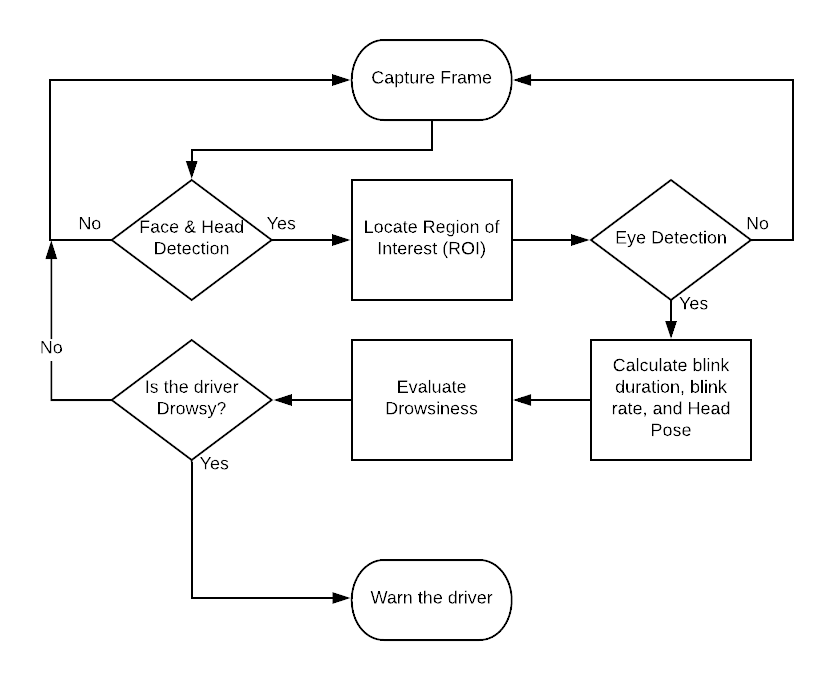
\includegraphics[scale=0.7]{EyeFlowchart}
	\caption{Eye Evaluation Flowchart}
\end{figure}


\end{center}

\begin{center}
	\begin{figure}[ht]
		\centering
		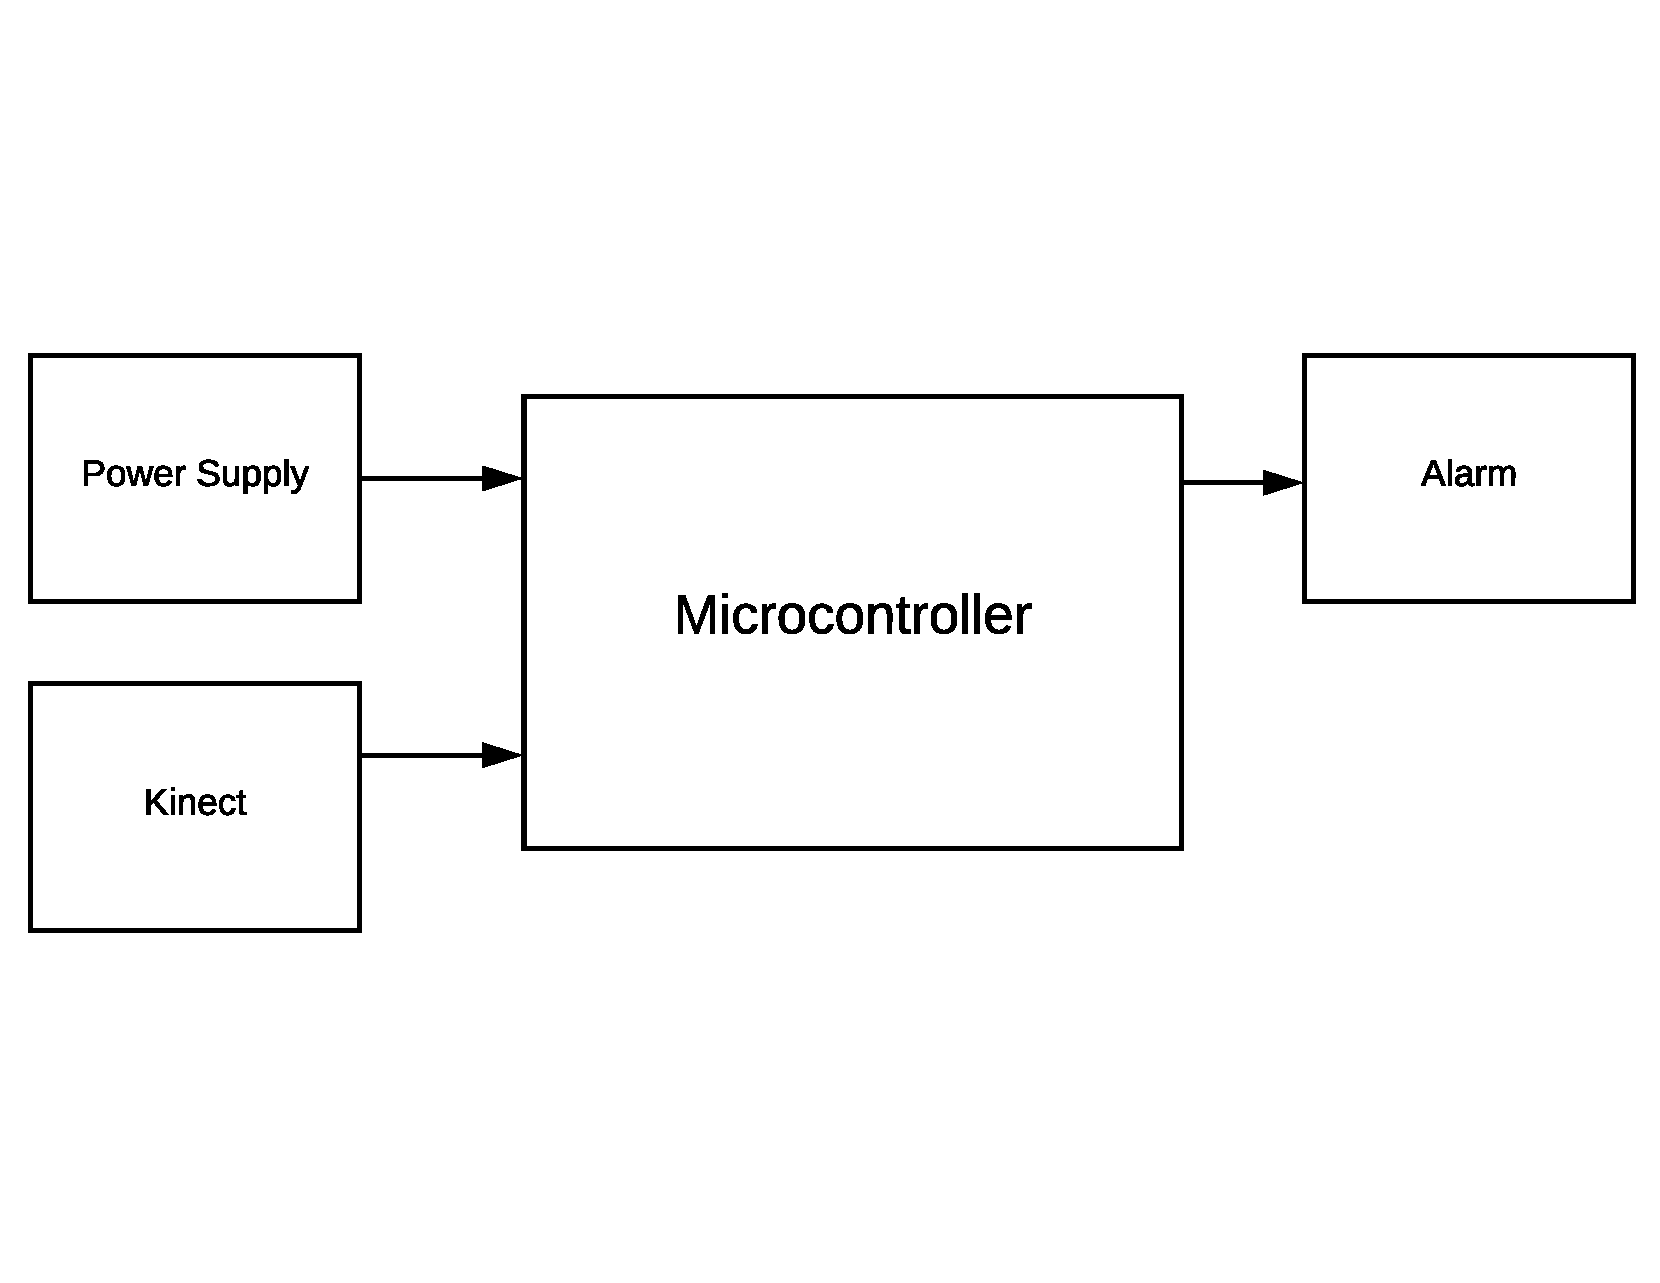
\includegraphics[scale=0.45]{BlockDiagram}
		\caption{Proposed Block Diagram of Driver Monitoring System}
	\end{figure}
\end{center}
\newpage
\section{Overview}

\subsection{Gantt Chart}
The following figures shown below is the individual gantt chart of the researchers:

\begin{figure}[!htb]
	\centering
	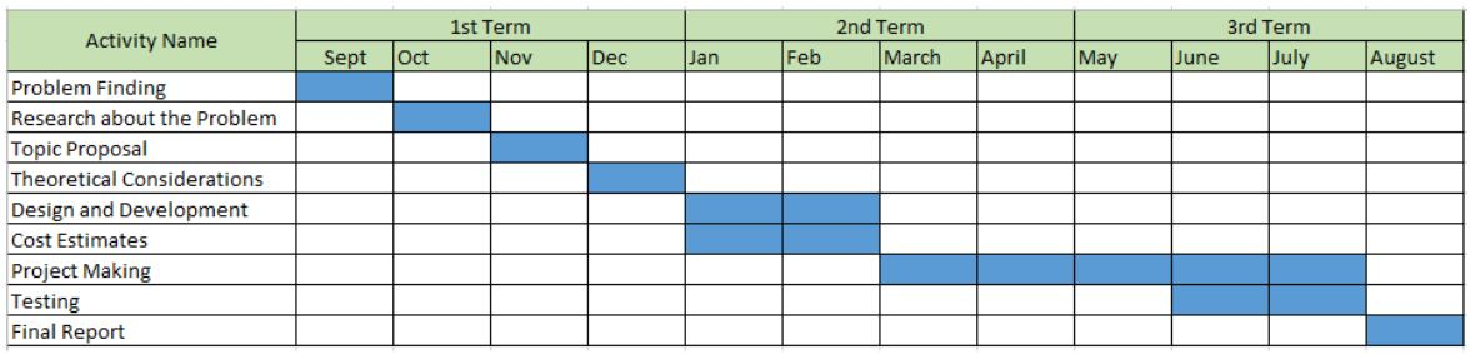
\includegraphics[scale=0.25]{gantt1}
	\caption{Gantt Chart of Guevarra}
\end{figure}
\begin{figure}[!htb]
	\centering
	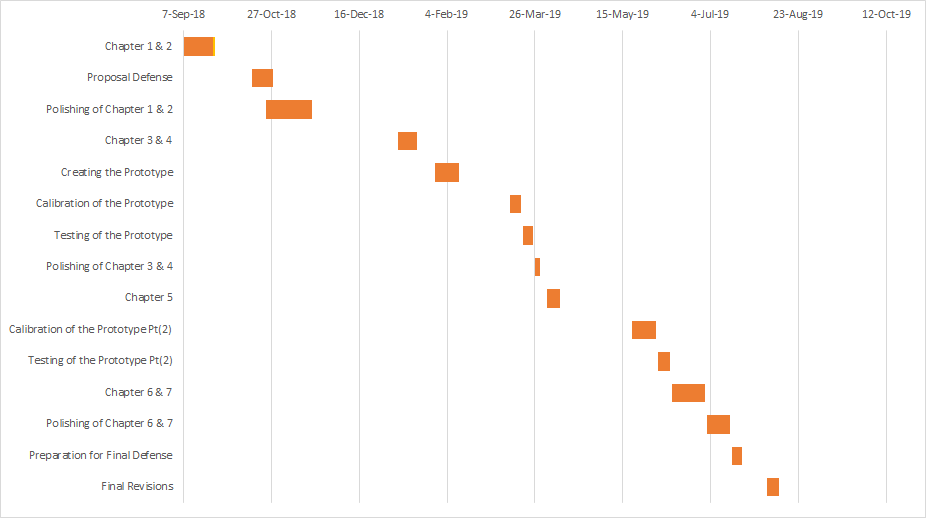
\includegraphics[scale=0.6]{gantt2}
	\caption{Gantt Chart of Hernandez}
\end{figure}
\begin{figure}[!htb]
	\centering
	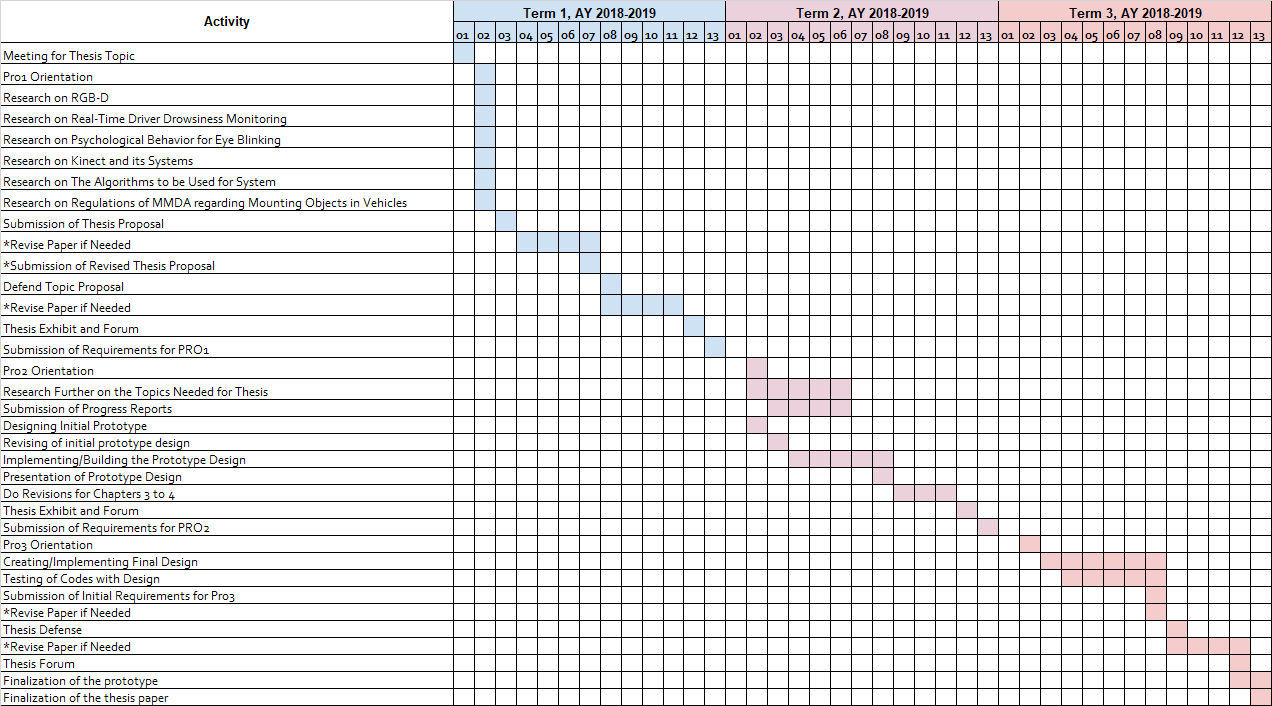
\includegraphics[scale=0.45]{gantt3}
	\caption{Gantt Chart of Lagman}
\end{figure}
\begin{figure}[!htb]
	\centering
	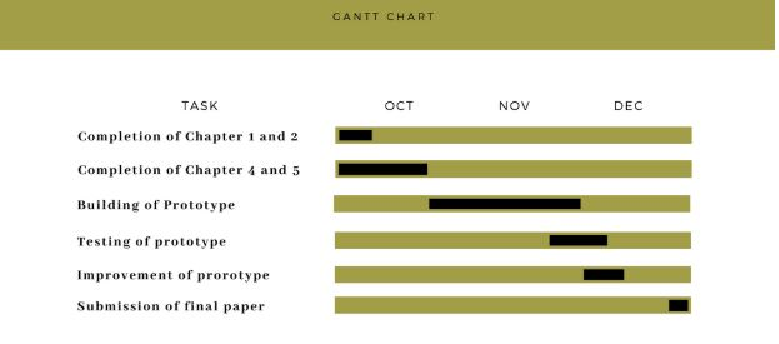
\includegraphics[scale=0.6]{gantt4}
	\caption{Gantt Chart of Villanueva}
\end{figure}
\newpage
\newpage
\subsection{Estimated Work Schedule and Budget}
\begin{table}[!htb]
	\caption{Price List of Materials to be Used}
	\centering
	\begin{tabular}{|c|c|}
		\hline
		Materials & Estimated Price(in PHP) \\
		\hline
		Kinect Sensor & 13.9k \\
		\hline
		Microcontroller & 21.2k \\
		\hline
		Laptop & Already Available \\
		\hline
		Total Price & 35.1k \\
		\hline
	\end{tabular}
\end{table}